\documentclass[]{standalone}

\usepackage{../lenses}

%\usetikzlibrary {shapes.geometric, math}
\usetikzlibrary{calc,math}

\newcommand{\starGeneric}[5]{ % symm,angle1,side,color,rot
 \tikzmath{
  \n      = int(#1)-1;
  \angle  = 180/#1;
  \angleA = #2*\angle;
  \angleB = 180 -\angle -\angleA;
  \r = #3 * sin(\angleA) / sin(\angle);
  \R = #3 * sin(\angleB) / sin(\angle);
 }
 \path(0,-0.5) node[right]{$n=\n$};
 \path(0,-1.0) node[right]{$a_0=\angle, a_A=\angleA,a_B=\angleB$};
 \path(0,-1.5) node[right]{$s=#3, r=\r,R=\R$};
 \definecolor{main}{HTML}{#5}
 \begin{scope}[rotate=#4*180/#1,shift={(-\R,0)}]
  \fill[main, opacity=0.5, draw=black, thick]
   (0:\R)
   \foreach \i in {0,...,\n} { 
    -- (2*\i*\angle:\R) -- ({(2*\i+1)*\angle}:\r)
   }
   --cycle;
  \end{scope}
}

\begin{document}
 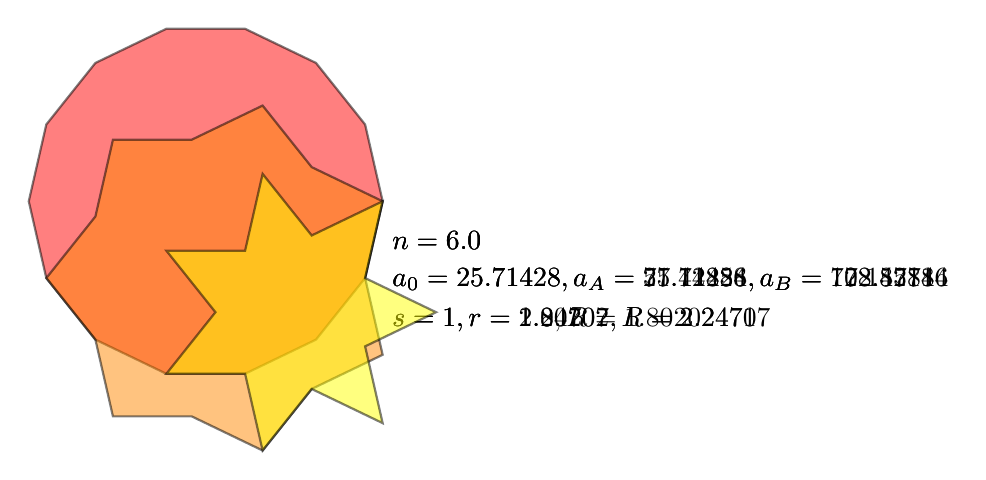
\begin{tikzpicture}
  \begin{scope}[scale=1]
   \starGeneric{7}{3}{1}{0}{FF0000}{0.5}
   \starGeneric{7}{2}{1}{1}{FF8800}{0.5}
   \starGeneric{7}{1}{1}{2}{FFFF00}{0.5}
  \end{scope}
 \end{tikzpicture}
\end{document}